\section{Visualisierung in Unity}
Dem Benutzer soll über eine geeignete Möglichkeit der aktuelle Spielstand wie auch die Suchresultate visualisiert
werden. Dazu wird wie bereits im Kapitel \ref{sec:architecture} erwähnt, eine Applikation mithilfe der Engine Unity
erstellt. Die Applikation erfüllt mehrere Ziele:
\begin{description}
    \item[Darstellung des aktuellen Spielstands] Der aktuelle Spielstand wird dem Benutzer präsentiert. Es besteht die
    Möglichkeit, Kugeln auszuwählen und eine Suche über diese zu starten.
    \item[Darstellung des Suchergebnisses] Sobald eine Suche durchgeführt wurde und Ergebnisse vorliegen, können diese
    über eine Animation angezeigt werden.
    \item[Erstellen neuer Spielstände] Als Zusatz wird eine Möglichkeit geschaffen, um Spielstände manuell zu generieren.
    Dies wird ausschliesslich während der Entwicklung verwendet.
\end{description}

Die Visualisierung des aktuellen Spielstands kann in der Abbildung \ref{fig:unity:spielstand} entnommen werden.
Die Kugeln können ein- wie auch ausgeblendet werden. Dies ist ebenso mit dem Tisch möglich, der standardmässig nicht
angezeigt wird. In der Abbildung ist weiterhin ersichtlich, dass die Positionen der Kugeln angezeigt werden können.
Auch diese Information ist nur für die Entwicklung relevant.
\begin{figure}[h!]
    \begin{center}
        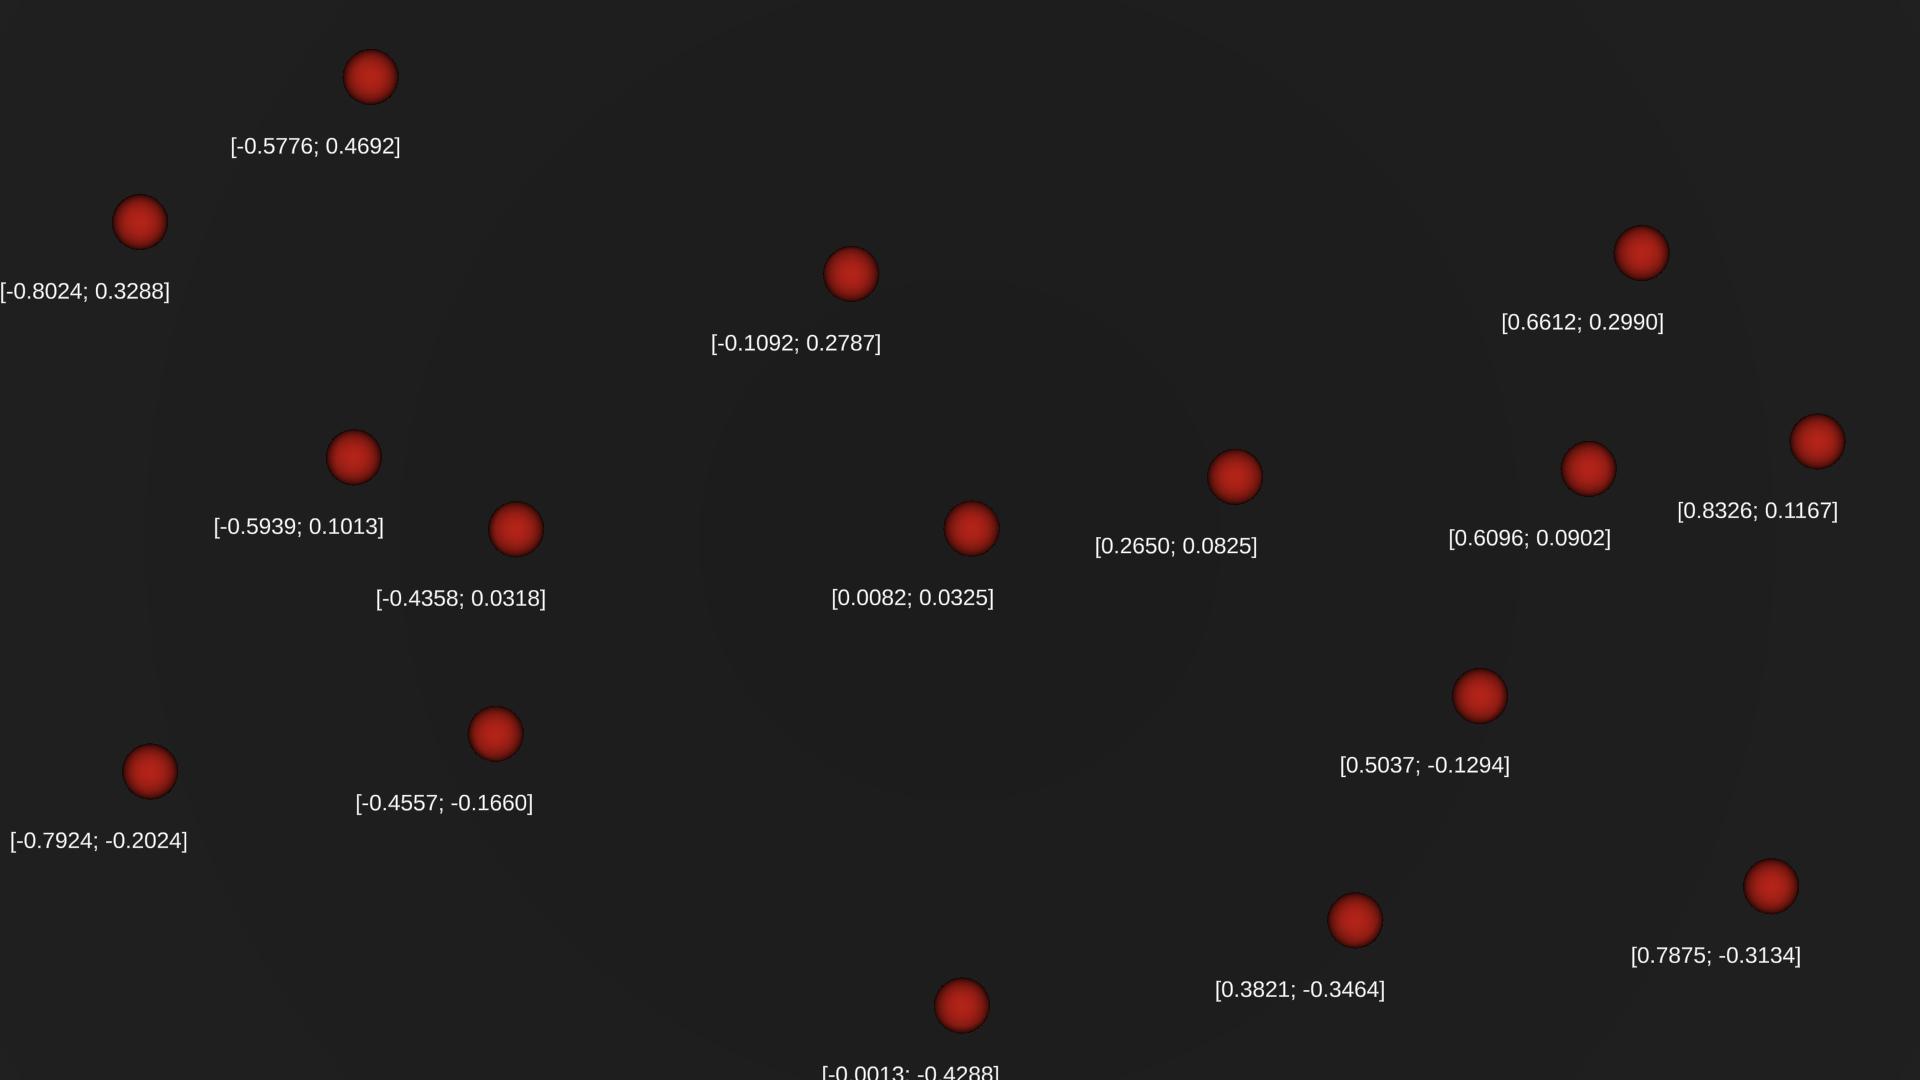
\includegraphics[width=0.7\linewidth]{../common/03_billiard_ai/resources/03_unity_spielstand.png}
    \end{center}
    \caption{Unity - Spielstand}
    \label{fig:unity:spielstand}
\end{figure}